\section{Introduction}
\label{sec:intro}
{\let\thefootnote\relax\footnote{{$^*$First two authors contributed equally to this work.}}}

Recent work has made substantial progress in fully automatic, 3D feature-based point cloud registration. At first glance, benchmarks like \textit{3DMatch}~\cite{zeng20163dmatch} appear to be saturated, with multiple state-of-the-art (SoTA) methods~\cite{gojcic20193DSmoothNet,Choy2019FCGF,bai2020d3feat} reaching nearly 95\% feature matching recall and successfully registering $>$80\% of all scan pairs.
One may get the impression that the registration problem is solved---but this is actually not the case. We argue that the high success rates are a consequence of lenient evaluation protocols. We have been making our task too easy:
existing literature and benchmarks~\cite{choi2015robust, zeng20163dmatch, khoury2017CGF} consider only pairs of point clouds with $\geq$30\% overlap to measure performance.
Yet, the low-overlap regime is very relevant for practical applications. On the one hand, it may be difficult to ensure high overlap, for instance when moving along narrow corridors, or when closing loops in the presence of occlusions (densely built-up areas, forest, etc.). On the other hand, data acquisition is often costly, so practitioners aim for a low number of scans with only the necessary overlap~\cite{yang2019extreme,yang2020extreme}. 

\begin{figure}[t]
    \centering
    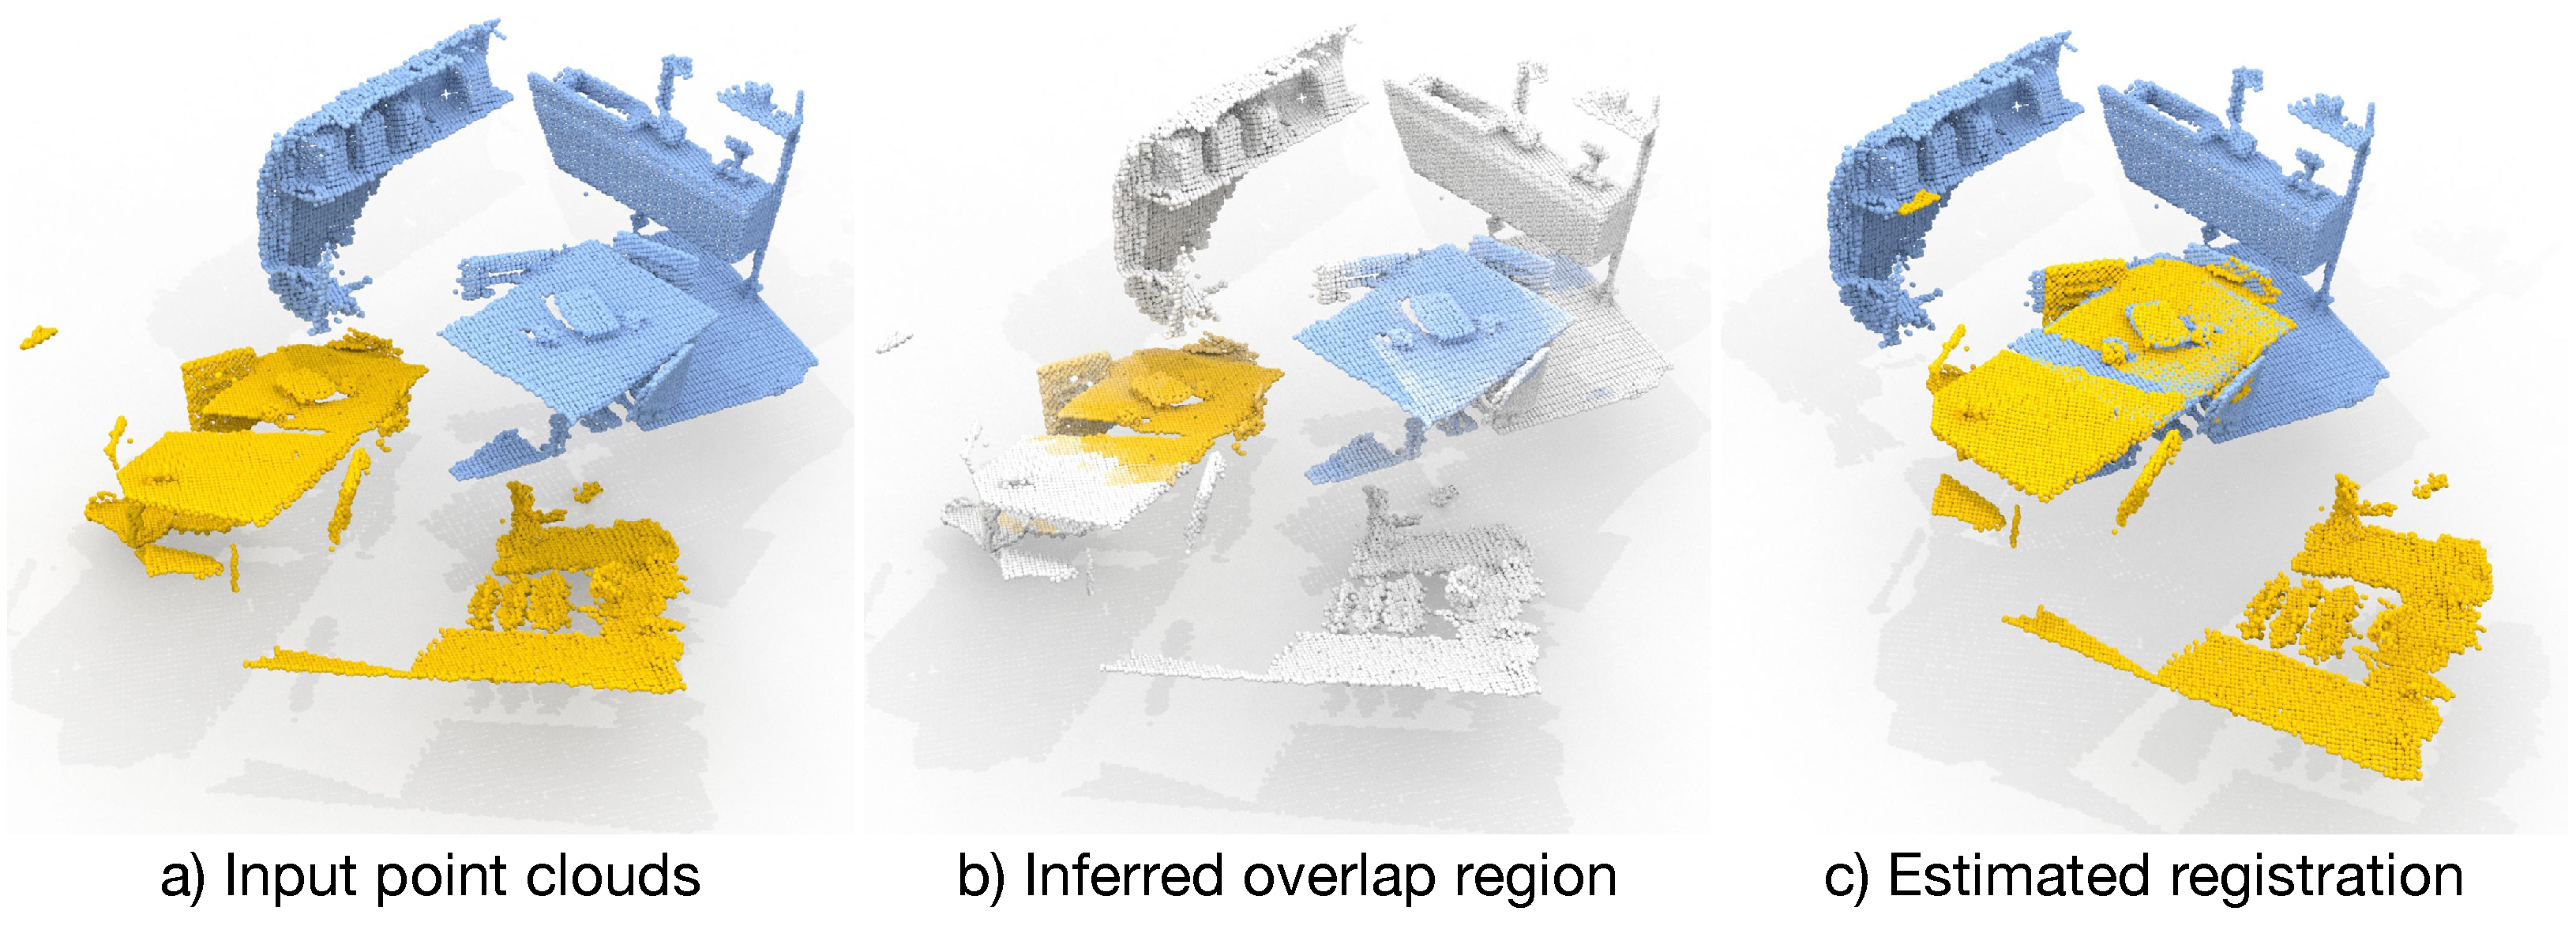
\includegraphics[width=1.0\columnwidth]{figures/images/teaser.pdf}
    \caption{\acro\ is designed to focus attention on the overlap region, and to prefer salient points in that region, so as to enable robust registration in spite of low overlap.}
    \label{fig:teaser_image}
\end{figure}
Driven by the evaluation protocol, the high-overlap scenario became the focus of research, whereas the more challenging low-overlap examples were largely neglected~(\cf~Fig.~\ref{fig:teaser_image}).
Consequently, the registration performance of even the best known methods deteriorates rapidly when the overlap between the two point clouds falls below 30\%, see Fig.~\ref{fig:motivation}.
Human operators, in contrast, can still register such low overlap point clouds without much effort.%

This discrepancy is the starting point of the present work. %
To %
study its reasons, we have constructed a low-overlap dataset \textit{3DLoMatch} from scans of the popular \textit{3DMatch} benchmark, and have analysed the individual modules/steps of the registration pipeline (Fig.~\ref{fig:motivation}).
It turns out that the effective receptive field of fully convolutional feature point descriptors~\cite{Choy2019FCGF,bai2020d3feat} is local enough and the descriptors are hardly corrupted by non-overlapping parts of the scans. Rather than coming up with yet another way to learn better descriptors, the key to registering low overlap point clouds is \emph{learning where to sample feature points}. A large performance boost can be achieved if the feature points are predominantly sampled from the overlapping portions of the scans~(Fig.~\ref{fig:motivation}, right).

We follow this path and introduce \acro,
a neural architecture for pairwise 3D point cloud registration that learns to detect the overlap region between two unregistered scans, and to focus on that region when sampling feature points.
The main contributions of our work are:
\begin{itemize}
    \item an analysis why existing registration pipelines break down in the low-overlap regime
    \item a novel \emph{overlap attention} block that allows for early information exchange between the two point clouds and focuses the subsequent steps on the overlap region
    \item a scheme to refine the feature point descriptors, by conditioning them also on the respective other point cloud
    \item a novel loss function to train \emph{matchability} scores, which help to sample better and more repeatable interest points
\end{itemize}
Moreover, we make available the \textit{3DLoMatch} dataset, containing the previously ignored scan pairs of \textit{3DMatch} that have low (10-30\%) overlap.
In our experiments, \acro\ greatly outperforms existing methods in the low-overlap regime, increasing registration recall by \textgreater15 percent points.
It also sets a new state of the art on the \textit{3DMatch} benchmark, reaching a registration recall of \textgreater90\%.
